\subsection[Correction to $dN/dn_{ch}$]{Correction to $\mathbf{dN/dn_{ch}}$}\label{section:star_dNdnch}

The observed $n_{sel}$ distribution is first corrected for the vertex reconstruction efficiency.  To remove the detector effects in the final results, one needs to express the multiplicity distribution in terms
of the number of charged primary particles $n_{ch}$ instead of the number of selected charged tracks $n_{sel}$. For
this, a Bayesian unfolding procedure is used \cite{DAGOSTINI1995487}. Integrating the probability relation given by the Bayes
theorem $P(n_{ch})\cdot P(n_{sel}|n_{ch}) = P(n_{ch}|n_{sel})\cdot P(n_{sel})$ over $n_{sel}$, one gets the distribution of primary particles:
\begin{equation}
\begin{array}{ccccc}
N_{ev}(n_{ch})&=&&\sum_{n_{sel}\geq0}P(n_{ch}|n_{sel})\cdot N_{ev}(n_{sel})\\
&=&\frac{1}{\epsilon^{miss}(n_{ch})}&\sum_{n_{sel}\geq2}P(n_{ch}|n_{sel})\cdot N_{ev}(n_{sel})
\end{array}
\end{equation}
The second relation factorizes the contribution of events that are lost due to track reconstruction inefficiency
but would pass the particle level phase-space cuts, i.e. those with $n_{ch}\geq2$ but $n_{sel}<2$. They are corrected
for by a special factor $\epsilon^{miss}(n_{ch})$ shown in the Fig. (referencja). The unfolding procedure is done iteratively to improve the estimate of $P(n_{ch}|n_{sel})$ taken from the MC:
\begin{itemize}
	\item First iteration: \\
	\begin{eqnarray}
	P(n_{ch}|n_{sel}) = P = P(n_{sel}|n_{ch})\frac{P^{MC}(n_{ch})}{P^{MC}(n_{sel})}
	\end{eqnarray}
	\begin{equation}
	N_{ev}(n_{ch})=\frac{1}{\epsilon^{miss}(n_{ch})}\sum_{n_{sel}\geq2}N_{ev}^{MC}(n_{sel})\cdot P
	\end{equation}
	where the resolution function $P(n_{sel}|n_{ch})$ is obtained from MC (number of tracks corresponding to a given number of particles).
	
	\item Next iterations $r+1$:
	\begin{equation}
	P^{r+1}=P(n_{sel}|n_{ch})\frac{P^{r}(n_{ch})}{P^{r}(n_{sel})}
	\end{equation}
	where normalized $N_{ev}^r(n_{ch})$ and $N_{ev}^r(n_{sel})$ serve as probability distributions $P^{r}(n_{ch})$ and $P^{r}(n_{sel})$.
\end{itemize}

This matrix shown in Fig. ?? is obtained using Monte Carlo and is applied to data to obtain the observed $n_{ch}$ distribution. While the matrix is mostly populated along the diagonal, it shows events with large multiplicity at particle
level, reconstructed with significantly smaller multiplicity at detector level. The total number of events, $N_{ev}$, is defined as the integral of the unfolded $N_{ch}$ distribution.
\captionsetup{format=plain,indention=0pt,justification=justified}
\begin{figure}[h!]
	\centering
	\begin{subfigure}{.49\textwidth}
		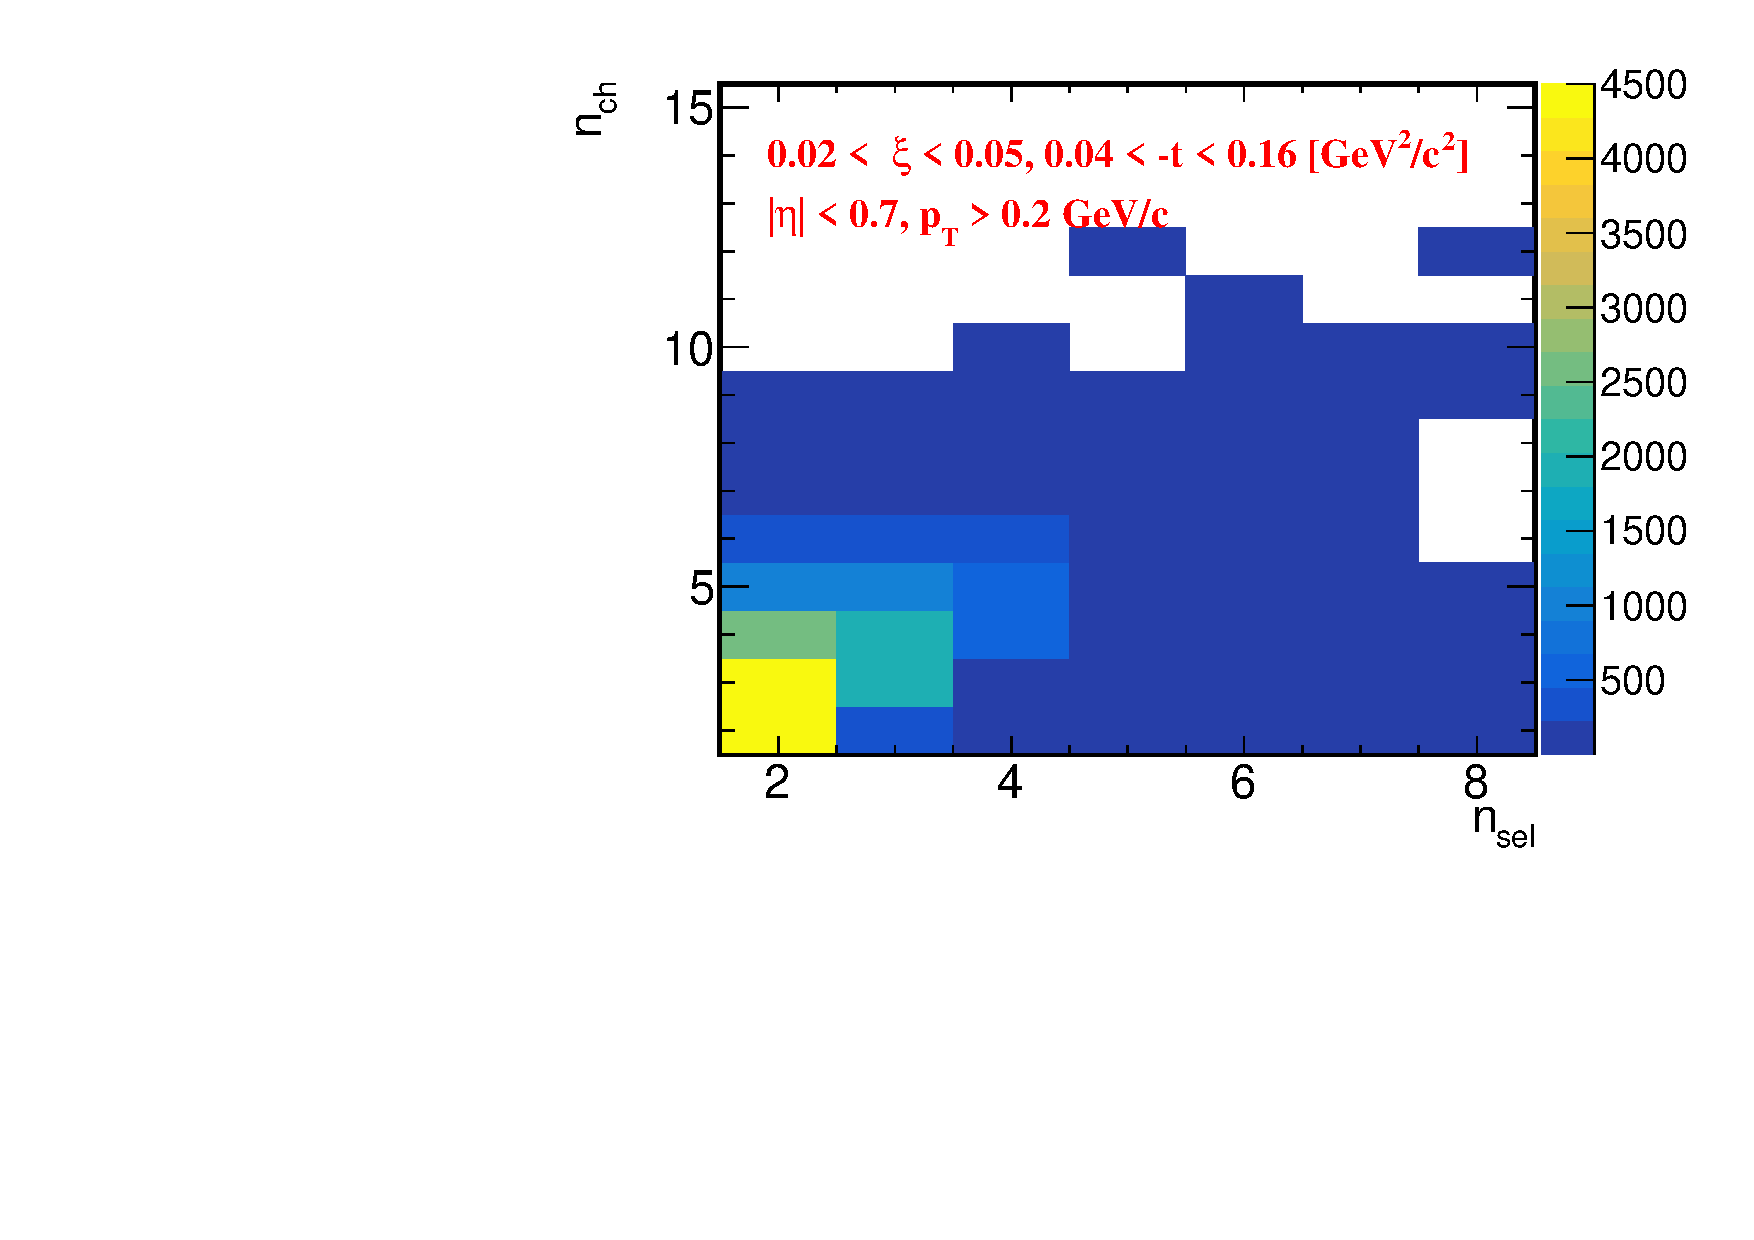
\includegraphics[width=\textwidth,page=1]{chapters/chrgSTAR/img/unfolding/matrix_0.pdf}
	\end{subfigure}
	\begin{subfigure}{.49\textwidth}
		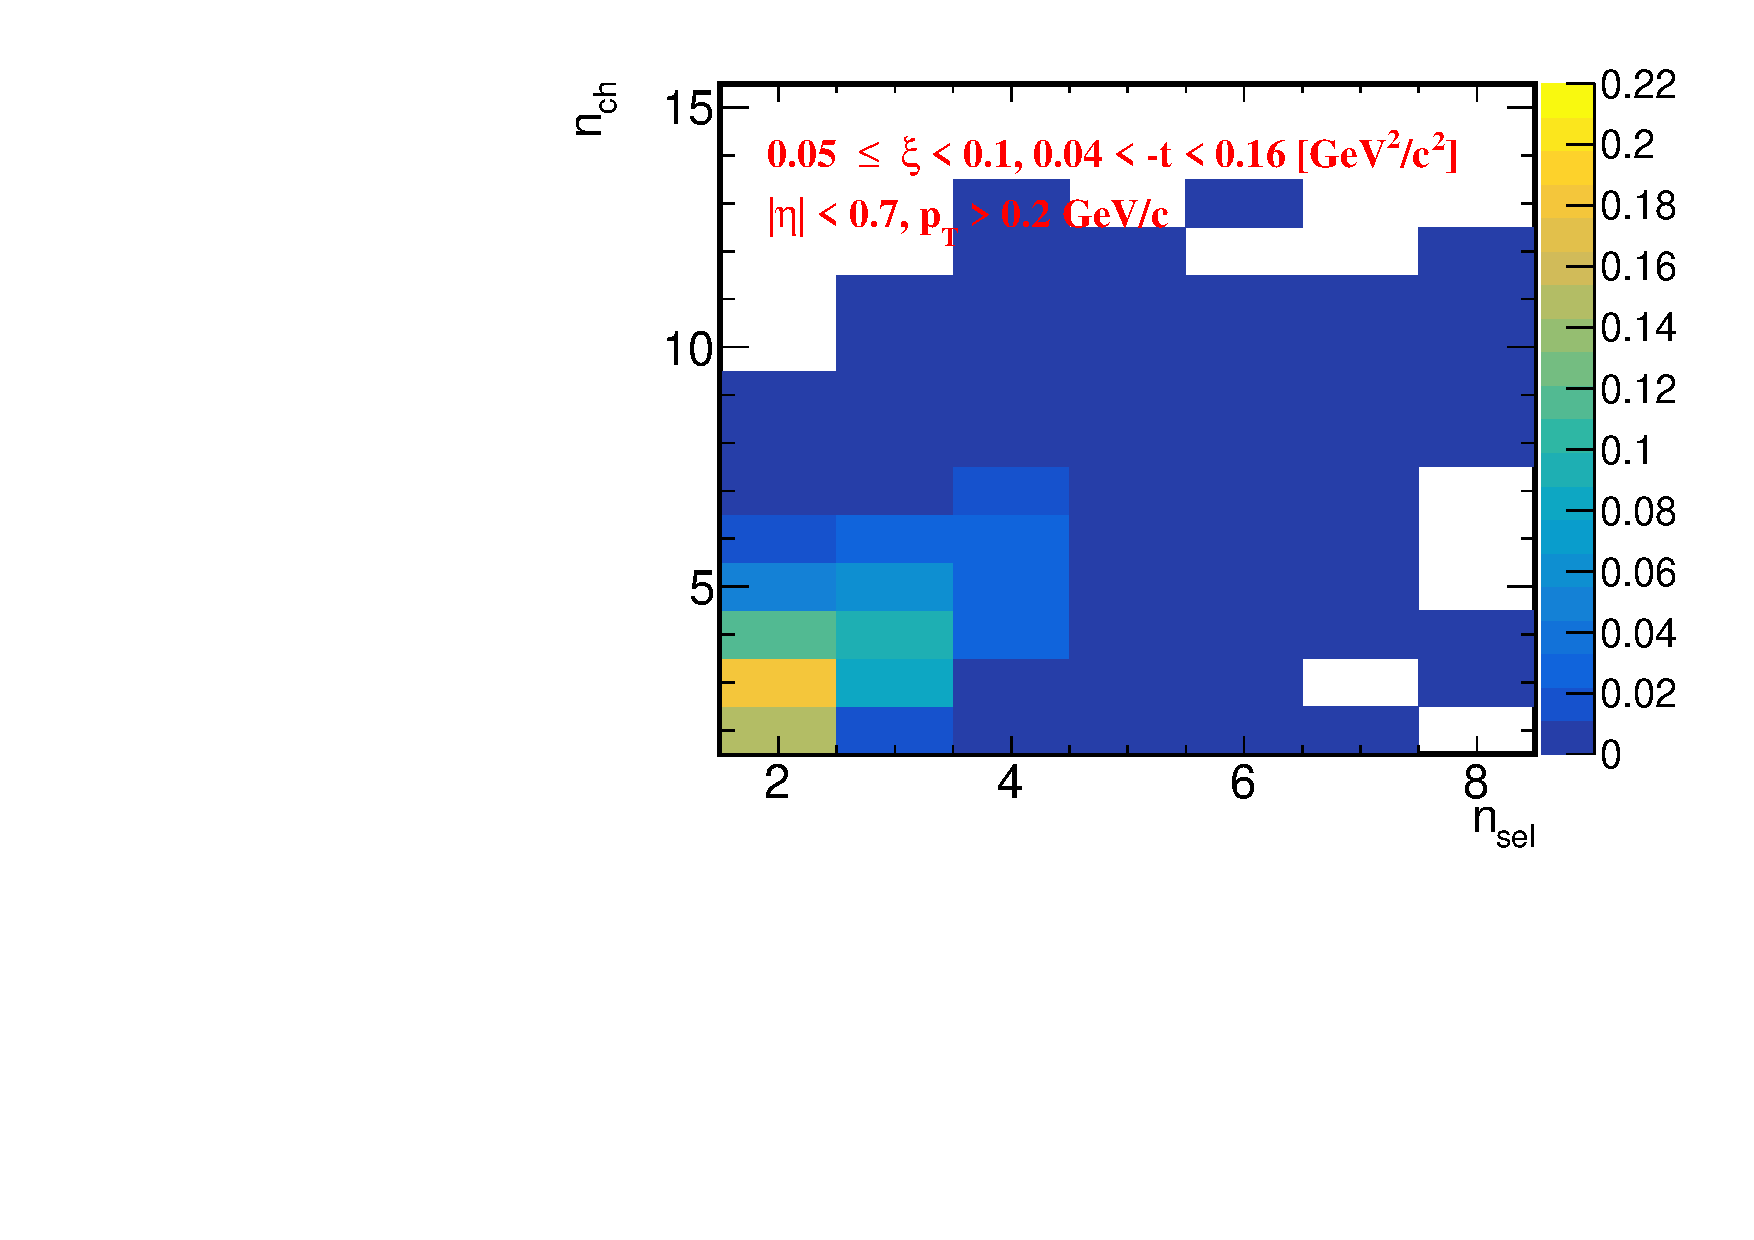
\includegraphics[width=\textwidth,page=1]{chapters/chrgSTAR/img/unfolding/matrix_1.pdf}
	\end{subfigure}
	\begin{subfigure}{.49\textwidth}
		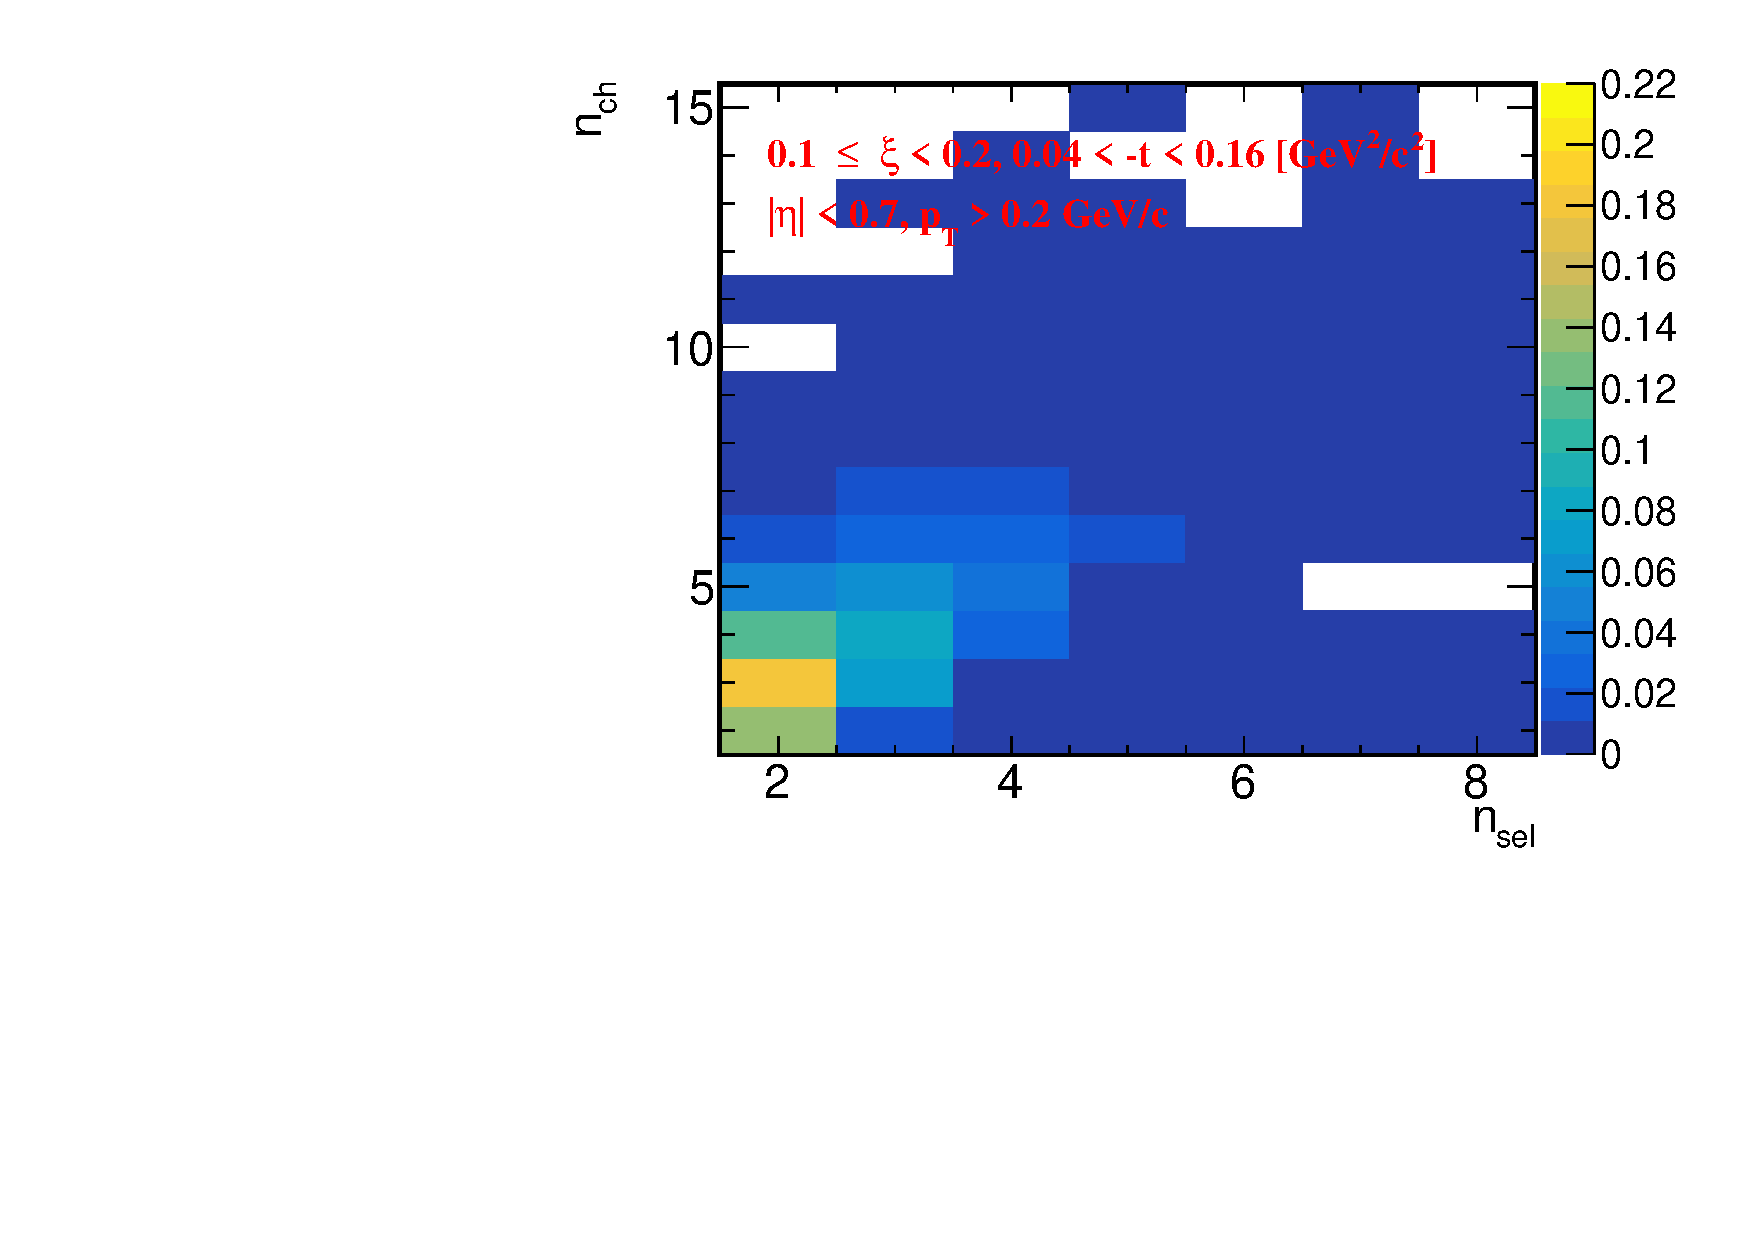
\includegraphics[width=\textwidth,page=1]{chapters/chrgSTAR/img/unfolding/matrix_2.pdf}
	\end{subfigure}
	\begin{minipage}{.49\textwidth}
		\caption{}
		\label{fig:responseSTAR}
	\end{minipage}
\end{figure}
\captionsetup{format=default,indention=0pt,justification=justified}